\section{Transportation model}
A transportation modelling is method for determining a traffic on road in focused area. Our goal is determine number of trip per road in road network from socio-economic and demographic data.

Traditional transportation modelling have a several independent step (e.g trip generation, trip destination, ...). Our implementation of transportation modelling consist from 3 steps.
\begin{itemize}
\item[ ] \textbf{trip generation} - I this part we want to determine number of trip origin, destination in zones. This step is depend on data (e.g demographic data, socio-economic data, weather, local habits, ...). Quality of model depend a lot on these data.
\item[ ] \textbf{trip destination} - In this section we want determine \textit{transportation matrix} $T$ (OD matrix). It say how many people travel from zone $i$ to zone $j$. For it was used Gravity model.
\item[ ] \textbf{counting traffic} - This is last step.  We compute traffic for every road link (edge of graph).
\end{itemize}
In upcoming section following expressions will be used:

\begin{tabular}{ll}
$T$ & transportation matrix (number of trips between zones)\\
$C$ & travel cost matrix (between zones) \\
$T_i, T_j$ & sum value in row/column in $T$\\
$n$ & number of zones (size of matrix)
\end{tabular}

\subsection{Trip destination}

For determine transportation matrix $T$ was used Gravity model:
$$T_{ij} = K_i K_j T_i T_j f(C_{ij})$$
where
$$T_i = \sum_{j = 1}^{n} T_{ij}$$
$$T_j = \sum_{i = 1}^{n} T_{ij}$$
$$K_i = \frac{1}{\sum_{j} K_j T_j f(C_{ij})}$$
$$K_j = \frac{1}{\sum_{i} K_i T_i f(C_{ij})}$$
where in our case $$f(x) = x^{-2}$$
$T_i$ is number of trips outcoming from the zone (origin in the zone) $i$, $T_j$ is number of trips incoming to the zone (destination in zone) $j$. So sometimes transportation matrix is called \textit{OD Matrix}. 

Now we must determine $K_i$ and $K_j$. We used iterative proportional fitting. It is iterative solution. First we compute $T^1$ with $K_i, K_j = 1$. After we can use iteration equation for $T$:
$$T_{ij}^{p} = \frac{Z_i}{T_i^{m-1}} T_{ij}^{k-1}$$
$$T_{ij}^{k} = \frac{Z_j}{T_j^{m-1}} T_{ij}^{p}$$
where $Z_i$ and $Z_j$ are origin and destination trips (we know), $k$ is iteration.

For example:
$$Z = (\begin{array}{ccc}
24  & 34  & 15\\
\end{array})$$
$$
C = \left(\begin{array}{ccc}
0& 10 &20 \\
10& 0 &15 \\
20 & 15& 0 \\
\end{array}\right) \Rightarrow T^0 = \left(\begin{array}{ccc}
       0  & 8.16000  &  0.90000\\
   8.16000  &     0  & 2.26667\\
   0.90000  & 2.26667  &    0\\
\end{array}\right) \Rightarrow$$
$$T^0 = \left(\begin{array}{ccc}
       0  & 8.16000  &  0.90000\\
   8.16000  &     0  & 2.26667\\
   0.90000  & 2.26667  &    0\\
\end{array}\right) \Rightarrow T^1 = \left( \begin{array}{ccc}
    0.00000 &  22.71648 &   3.65832 \\
   20.68579 &   0.00000 &  11.34168 \\
    3.31421 &  11.28352 &   0.00000 \\
\end{array} \right)$$
After 1 iteration coefficients are:
$$\frac{Z_i}{\sum_j T_{ij}} = \left(\begin{array}{c}
0.90996 \\
1.06159  \\
1.02756\\
\end{array}\right) \quad \frac{Z_j}{\sum_i T_{ij}} = \left(\begin{array}{ccc}
0  & 0 & 0\\
\end{array}\right)$$


\subsection{Count traffic}
Now we know how many people travel from zone $i$ to zone $j$, so we can find path from $i$ to $j$ and 
record this value into every edges in path. So we have to compute $z^2$ shortest paths ($z$ is number of zones). Because we have to compute shortest path between all pair of zones.

In our solution we compute N paths for every pair of zones (finally will be compute $N z^2$ paths). Every path is based on another cost. Cost is based on length, time and vertical distance. Final cost is linear combination these partition cost.
$$c = \left(\begin{array}{ccc}
k_t & k_l & k_h\\
\end{array}\right) \left( \begin{array}{c}
t\\
l\\
h\\
\end{array} \right)$$

where $c$ is cost, $t$ is time, $l$ is length and $h$ is vertical distance. Number of trip (traffic between two zones) is splitted between those paths. In Fig. \ref{img.paths} you can see multipath (same pareto optimal paths) between two zones.
\begin{figure}
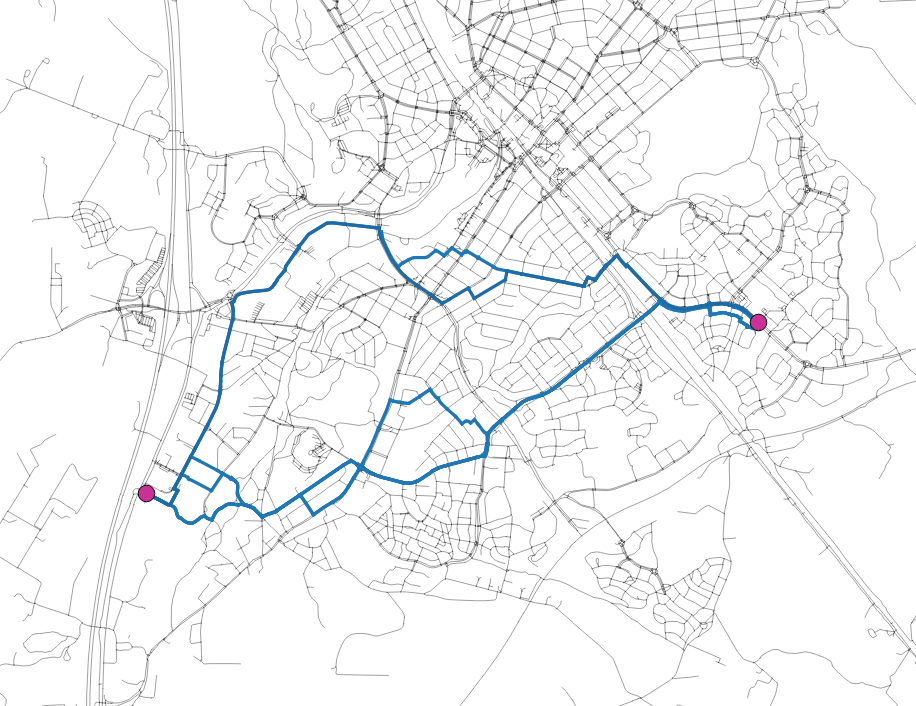
\includegraphics[width=12cm]{img/c01-transp-model/paths.png}
\label{img.paths}
\caption{Possible paths between one pair of zone (multipath)}
\end{figure}